\label{sterowniki}
W rozdziale \ref{pierwsze_uruchomienie_aktualizacja_instalacja} ,,Instalacja dodatkowych sterowników'' opisana została metoda instalacji dodatkowych sterowników. Często w ten sposób instaluje się właśnie sterowniki do kart graficznych. Jednak skoro komputer wyświetla obraz jeszcze przed instalacją tych modułów, to znaczy, że jakieś sterowniki muszą już wcześniej być obecne w systemie. Zgadza się. W Ubuntu domyślnie zainstalowane są sterowniki do niemalże każdej karty graficznej, rozwijane zgodnie z zasadami wolnego i~otwartego oprogramowania. Spotykają się one z różną reakcją producentów sprzętu. Niektórzy ten sposób dostarczania sterówników w pełni popierają i właśnie tak zapewniają oficjalne wsparcie dla Ubuntu, inni natomiast zupełnie go ignorują. Poza tymi, otwartoźródłowymi sterownikami niektórzy producenci sprzętu dostarczają też dla Ubuntu sterowniki oparte na zamkniętym (własnościowym) kodzie źródłowym. Są to na ogół swego rodzaju porty ich odpowiedników z windowsa, dzięki czemu zapewniają komplementarną wydajność i funkcjonalność. To właśnie takie sterowniki możesz doinstalować na zasadach opisanych w rozdziale poświęconym dodatkowym sterownikom. W tym rozdziale dowiesz się więcej o tym, z jakich sterowników powinieneś korzystać w swoim konkretnym przypadku.

\subsubsection{Identyfikacja karty graficznej i sterownika}
Żeby wiedzieć z jakich sterowników należy skorzystać, najpierw trzeba sprawdzić w jaki sprzęt wyposażony jest komputer. Część osób zapewne i bez żadnych dodatkowych procedur wie, jaką ma kartę graficzną, jednak żeby się upewnić, należy w terminalu wpisać:

\begin{lstlisting}[language=bash]
lspci | grep VGA
\end{lstlisting}
\begin{itemize}
\item \textcolor{ubuntu_orange}{lspci} --- program wyświetlający urządzenia obecne w komputerze;
\item \textcolor{ubuntu_orange}{$|$} --- ,,rura'', ,,pipe'', przekierowanie wyjścia z jednego programu na wejście drugiego;
\item \textcolor{ubuntu_orange}{grep} --- program wyszukujący wzorce;
\item \textcolor{ubuntu_orange}{VGA} --- szukany wzorzec, w tym wypadku szukamy urządzeń zgodnych ze standardem VGA (kart graficznych).
\end{itemize}

Wynik powyższej komendy zwróci producenta i nazwę karty graficznej, w jaką wyposażony jest komputer. Na przykład dla Nvidii:
\begin{lstlisting}[language=bash]
03:00.0 VGA compatible controller: NVIDIA Corporation G94 [GeForce 9600 GT] (rev a1)
\end{lstlisting}

Żeby dowiedzieć się z jakiego sterownika aktualnie korzysta twój komputer, należy wpisać komendę:

\begin{lstlisting}[language=bash]
glxinfo | grep OpenGL
\end{lstlisting}
\begin{itemize}
\item \textcolor{ubuntu_orange}{glxinfo} --- program wyświetlający surowe informacje o aktualnie działającym sterowniku do karty graficznej;
\item \textcolor{ubuntu_orange}{I} --- ,,rura'', ,,pipe'', przekierowanie wyjścia z jednego programu na wejście drugiego; 
\item \textcolor{ubuntu_orange}{grep} --- program wyszukujący wzorce;
\item \textcolor{ubuntu_orange}{OpenGL} --- szukany wzorzec, w tym wypadku szukamy informacji o zgodności z bibliotekami OpenGL.
\end{itemize}

Uwaga! Powyższa komenda wymaga zainstalowania pakietu ,,mesa-utils''. Pakiet ten domyślnie doinstalowuje się wraz z \textcolor{ubuntu_orange}{ubuntu-restricted-extras}, instalacja tej paczki jest opisana w rozdziale \ref{ubuntu-restricted-extras}. Jeżeli postępowałeś zgodnie z tamtymi wytycznymi, to nie musisz robić nic więcej, w przeciwnym przypadku odpowiedni pakiet należy zainstalować komendą:
\begin{lstlisting}[language=bash]
sudo apt-get install mesa-utils
\end{lstlisting}
\begin{itemize}
\item \textcolor{ubuntu_orange}{sudo} --- wykonuje dalsze polecenia z uprawieniami administratora systemu;
\item \textcolor{ubuntu_orange}{apt-get} --- program do zarządzania zainstalowanym oprogramowaniem;
\item \textcolor{ubuntu_orange}{install} --- informujesz apt, że chcesz zainstalować paczkę z oprogramowaniem;
\item \textcolor{ubuntu_orange}{mesa-utils} --- nazwa paczki do zainstalowania.
\end{itemize}

\subsubsection{Intel}
Karty graficzne produkowane przez Intela to w Ubuntu najprostszy przypadek. Intel oficjalnie rozwija jedynie otwarte sterowniki, które już są obecne zaraz po instalacji systemu. Żadne dodatkowe działanie użytkownika nie jest wymagane. Można dodatkowo zainstalować dwa pakiety, zapewniające akcelerację sprzetową podczas dekodowania filmów:

\begin{lstlisting}[language=bash]
sudo apt-get install i965-va-driver vainfo
\end{lstlisting}

\subsubsection{nVidia}
Na przeciwnym biegunie jest natomiast nVidia. Ten producent prawie zupełnie ignoruje otwarte sterowniki, ale za to dostarcza wysokiej jakości zamknięte moduły. Instaluje się je zgodnie z rozdziałem \ref{pierwsze_uruchomienie_aktualizacja_instalacja} ,,Instalacja dodatkowych sterowników''. 

\begin{center}
	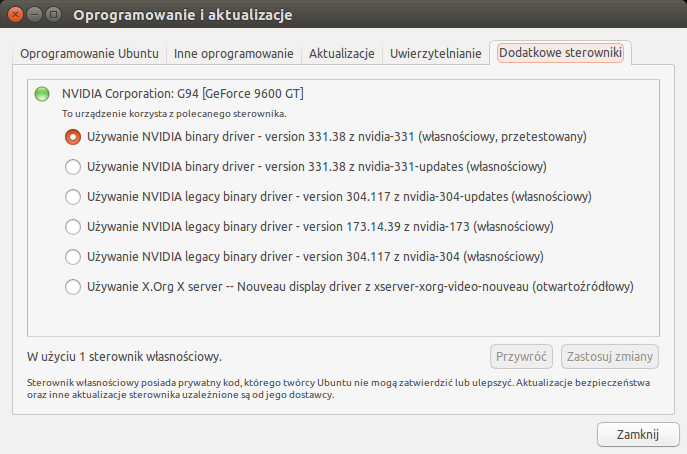
\includegraphics[width=\linewidth]{images/pierwsze_uruchomienie_driver2.png}
\end{center}

Do odpowiednich kart graficznych należy zainstalować sterowniki o wskazanych numerach:
\begin{itemize}
\item Sterownik 331.x do kart GeForce 8000 i nowszych;
\item Sterownik 304.x do kart 6000 -- 7000;
\item Sterownik 173.x do kart GeForce 5 (FX);
\item Sterownik 96.x do kart GeForce 4 i starszych.
\end{itemize}

Program instalujący dodatkowe sterowniki powinien poprawnie zidentyfikować kartę graficzną i~zaproponować odpowiednią wersję sterownika.
Akcelerację wideo poprzez VDPAU można doinstalować poleceniem:

\begin{lstlisting}[language=bash]
sudo apt-get install libvdpau1 vdpauinfo
\end{lstlisting}

Jeśli twój komputer to laptop z układem NVidia Optimus, a system nie rozpoznał tego układu, to może zajść potrzeba ręcznej instalacji pakietu nvidia-prime. 

\begin{lstlisting}[language=bash]
sudo apt-get nvidia-prime
\end{lstlisting}

\noindent Przełączanie układu graficznego wykonuje się w panelu ustawień \textcolor{ubuntu_orange}{nvidia-settings}.

Gdyby pakiet nvidia-prime nie działał poprawnie, można zamiast niego zainstalować Bumblebee. Ten program wyłącza dyskretną kartę NVidii, jednocześnie umożliwiając jej włączenie wtedy, gdy jest potrzebna.
Po wcześniejszym odinstalowaniu nvidia-prime, Bumblebee można zainstalować poleceniem:

\begin{lstlisting}[language=bash]
sudo apt-get install bumblebee bumblebee-nvidia
\end{lstlisting}

\subsubsection{AMD}
AMD w kwestii sterowników wybrało podejście pośrednie pomiędzy sposobem Intela, a nVidii. Z~jednej strony ten producent dostarcza zamknięte sterowniki (ale tylko do najnowszych kart graficznych), z drugiej zaś rozwija sterowniki otwarte, obsługujące starsze modele. Jeżeli jesteś użytkownikiem karty graficznej AMD Radeon HD 5000 lub nowszej, powinieneś zainstalować sterownik zamknięty, zgodnie z procedurą opisaną w rozdziale \ref{pierwsze_uruchomienie_aktualizacja_instalacja} ,,Instalacja dodatkowych sterowników''. W przypadku posiadania starszej karty graficznej, pozostaje użycie otwartego sterownika.

\begin{center}
	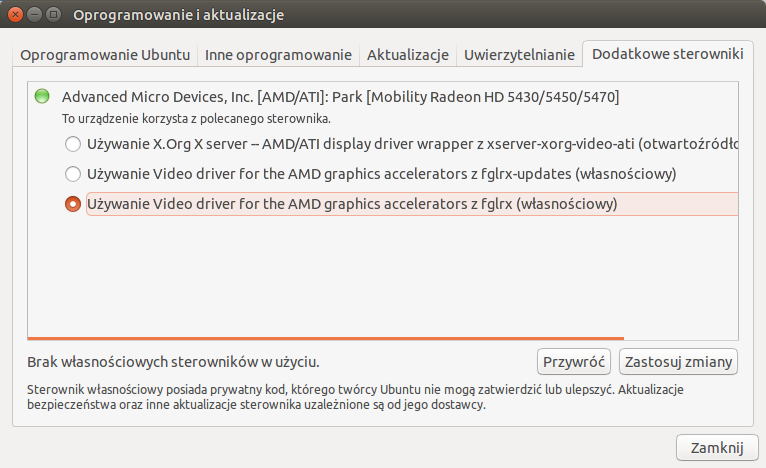
\includegraphics[width=\linewidth]{images/sterowniki_AMD.png}
\end{center}

W tym drugim wypadku można zapewnić akcelerację wideo poprzez VDPAU instalując pakiety poleceniem:
\begin{lstlisting}[language=bash]
sudo apt-get install libvdpau1 vdpauinfo mesa-vdpau-drivers
\end{lstlisting}

Posiadacze hybrydowych układów AMD powinni zainstalować paczki fglrx oraz fglrx-pxpress:

\begin{lstlisting}[language=bash]
sudo apt-get install fglrx fglrx-pxpress
\end{lstlisting}
